\section{Arquitectura}
La estructura general del programa se divide en los siguientes elementos:

\begin{figure}[h]
	\centering
		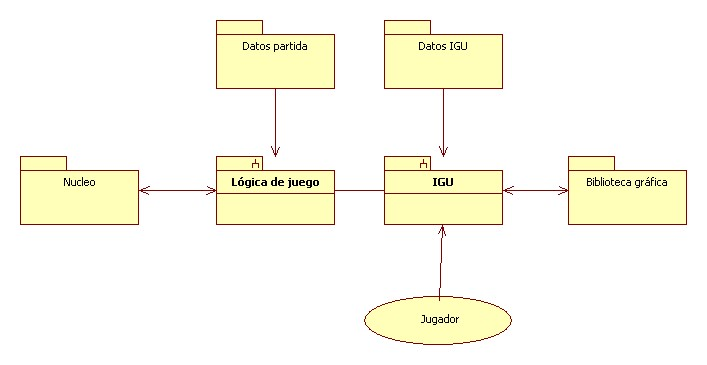
\includegraphics[width=15cm]{images/diagramas/arquitectura.jpg}
	\caption{Diagrama arquitectura}
	\label{fig:Arquitectura}
\end{figure}

\begin{itemize}
	\item \textbf{N�cleo}: Representa los diferentes m�dulos que constituyen en �ltimo t�rmino la l�gica de juego. Estos componentes reciben los datos proporcionados por el jugador y otros m�dulos y procesan en cada turno el siguiente estado de los mismos. El estado de dichos m�dulos es salvable y recuperable.
	\item \textbf{Biblioteca gr�fica}: Proporciona los componentes gr�ficos para el dibujado y la interacci�n con el interfaz de usuario 2D. Tambi�n proporciona mecanismo de control y comunicaci�n entre la parte gr�fica y la l�gica de juego.
	\item \textbf{Datos partida}: En primera instancia estos datos son le�dos de un fichero de configuraci�n XML y definen todas las caracter�sticas iniciales del estado a simular y, por consiguiente, el tipo de partida que el jugador va a experimentar.
	\item \textbf{Datos IGU}: En primera instancia estos datos son le�dos de un fichero de configuraci�n XML y definen todas las caracter�sticas iniciales del interfaz de usuario esto es, su apariencia, posici�n y tipo.
	\item \textbf{L�gica de juego}: Se encarga de controlar el juego sincronizando los diferentes m�dulos. Define cual es el orden de actualizaci�n de los m�dulos y por lo tanto de que manera se genera el siguiente estado en cada turno.
	\item \textbf{IGU}: Captura las entradas del usuario sobre el interfaz de usuario y las transforma de forma que sean elementos significativos para la l�gica de juego.
	\item \textbf{Jugador}: Representa al �nico jugador posible en un momento dado. HONOS es no es juego multijugador, por lo tanto todas las acciones provienen del mismo usuario para una misma partida.
\end{itemize}